\section{実験方法}
実験は事前準備と本実験の2段階で構成される．
本実験では，システムによる段階的な楽曲推薦を行う群（推薦あり群）と，支援を行わない群（推薦なし群）の2群で比較を行う．

\subsection{事前準備}

事前準備では，被験者に実験用のSpotifyアカウントを作成してもらい，50曲程度の「お気に入りの曲」プレイリストを作成する．その後，Webアプリケーションを用いて，図\ref{fig:song_classification}に示した楽曲分類画面で，各楽曲に対する思い入れの強さと歌唱への自信を4段階で評価する．ユーザーの作業の負担を考慮し，楽曲分類の際には途中で保存ができる機能を実装した．

また，図\ref{fig:classified_songs}に分類済みの楽曲一覧を確認できる画面を示す．この画面では，分類が完了した楽曲の一覧を表示する．被験者は，自身が分類した楽曲を確認することができる．また，再度の分類もできるようにした．

\begin{figure}[H]
   \centering
   \begin{minipage}[b]{0.45\linewidth}
       \centering
       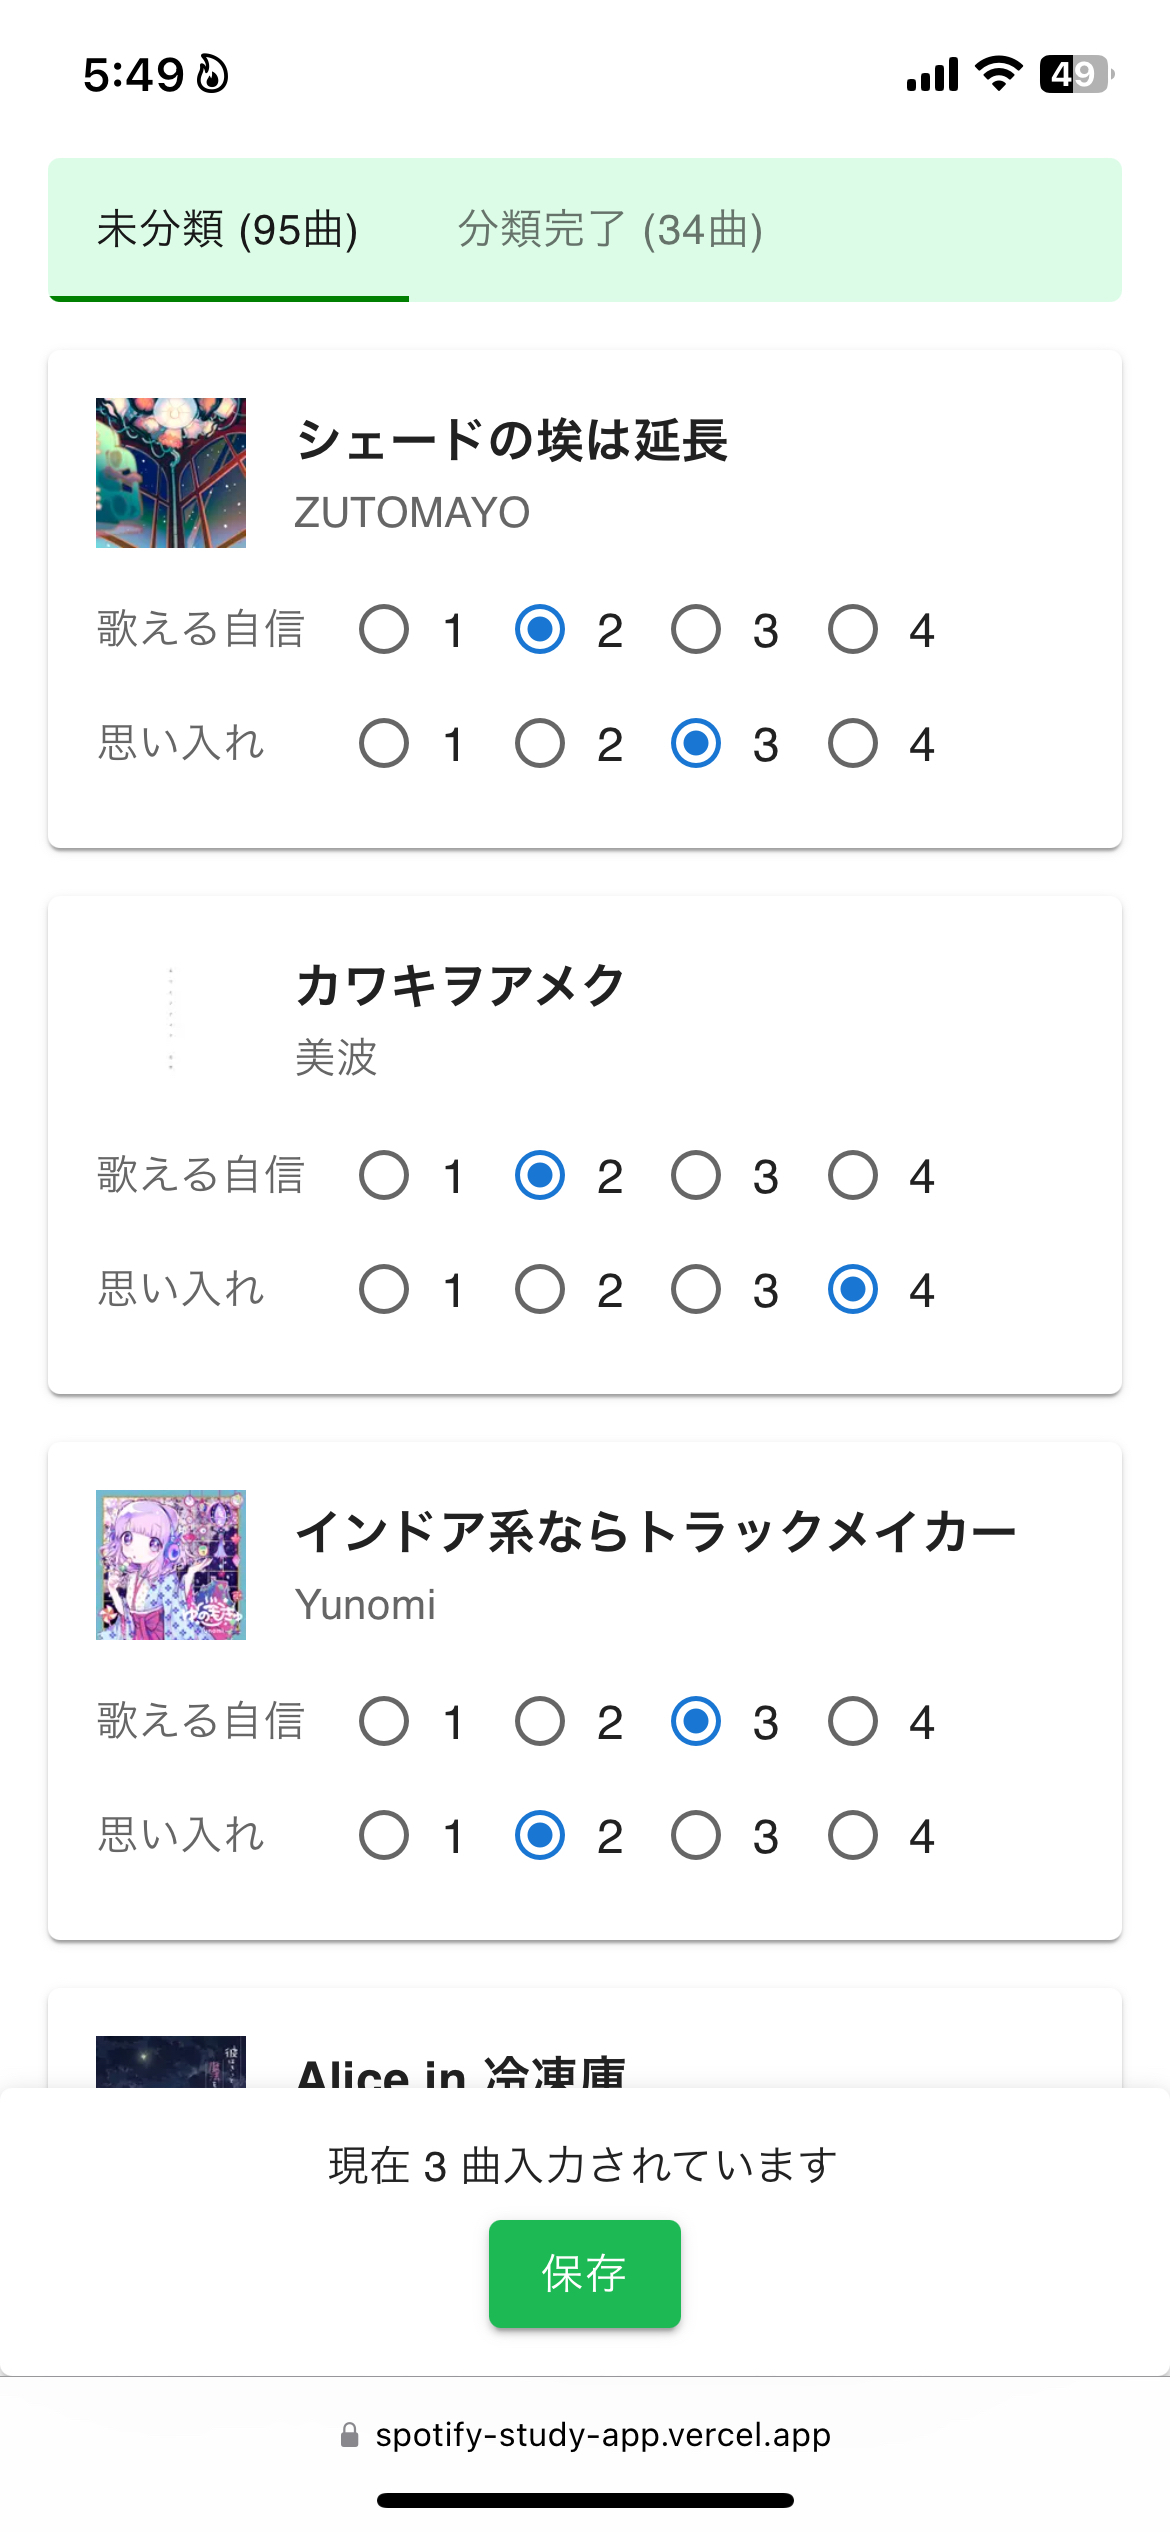
\includegraphics[width=0.9\linewidth]{image/ss_未分類.png}
       \caption{楽曲分類画面}
       \label{fig:song_classification}
   \end{minipage}
   \hfill
   \begin{minipage}[b]{0.45\linewidth}
       \centering
       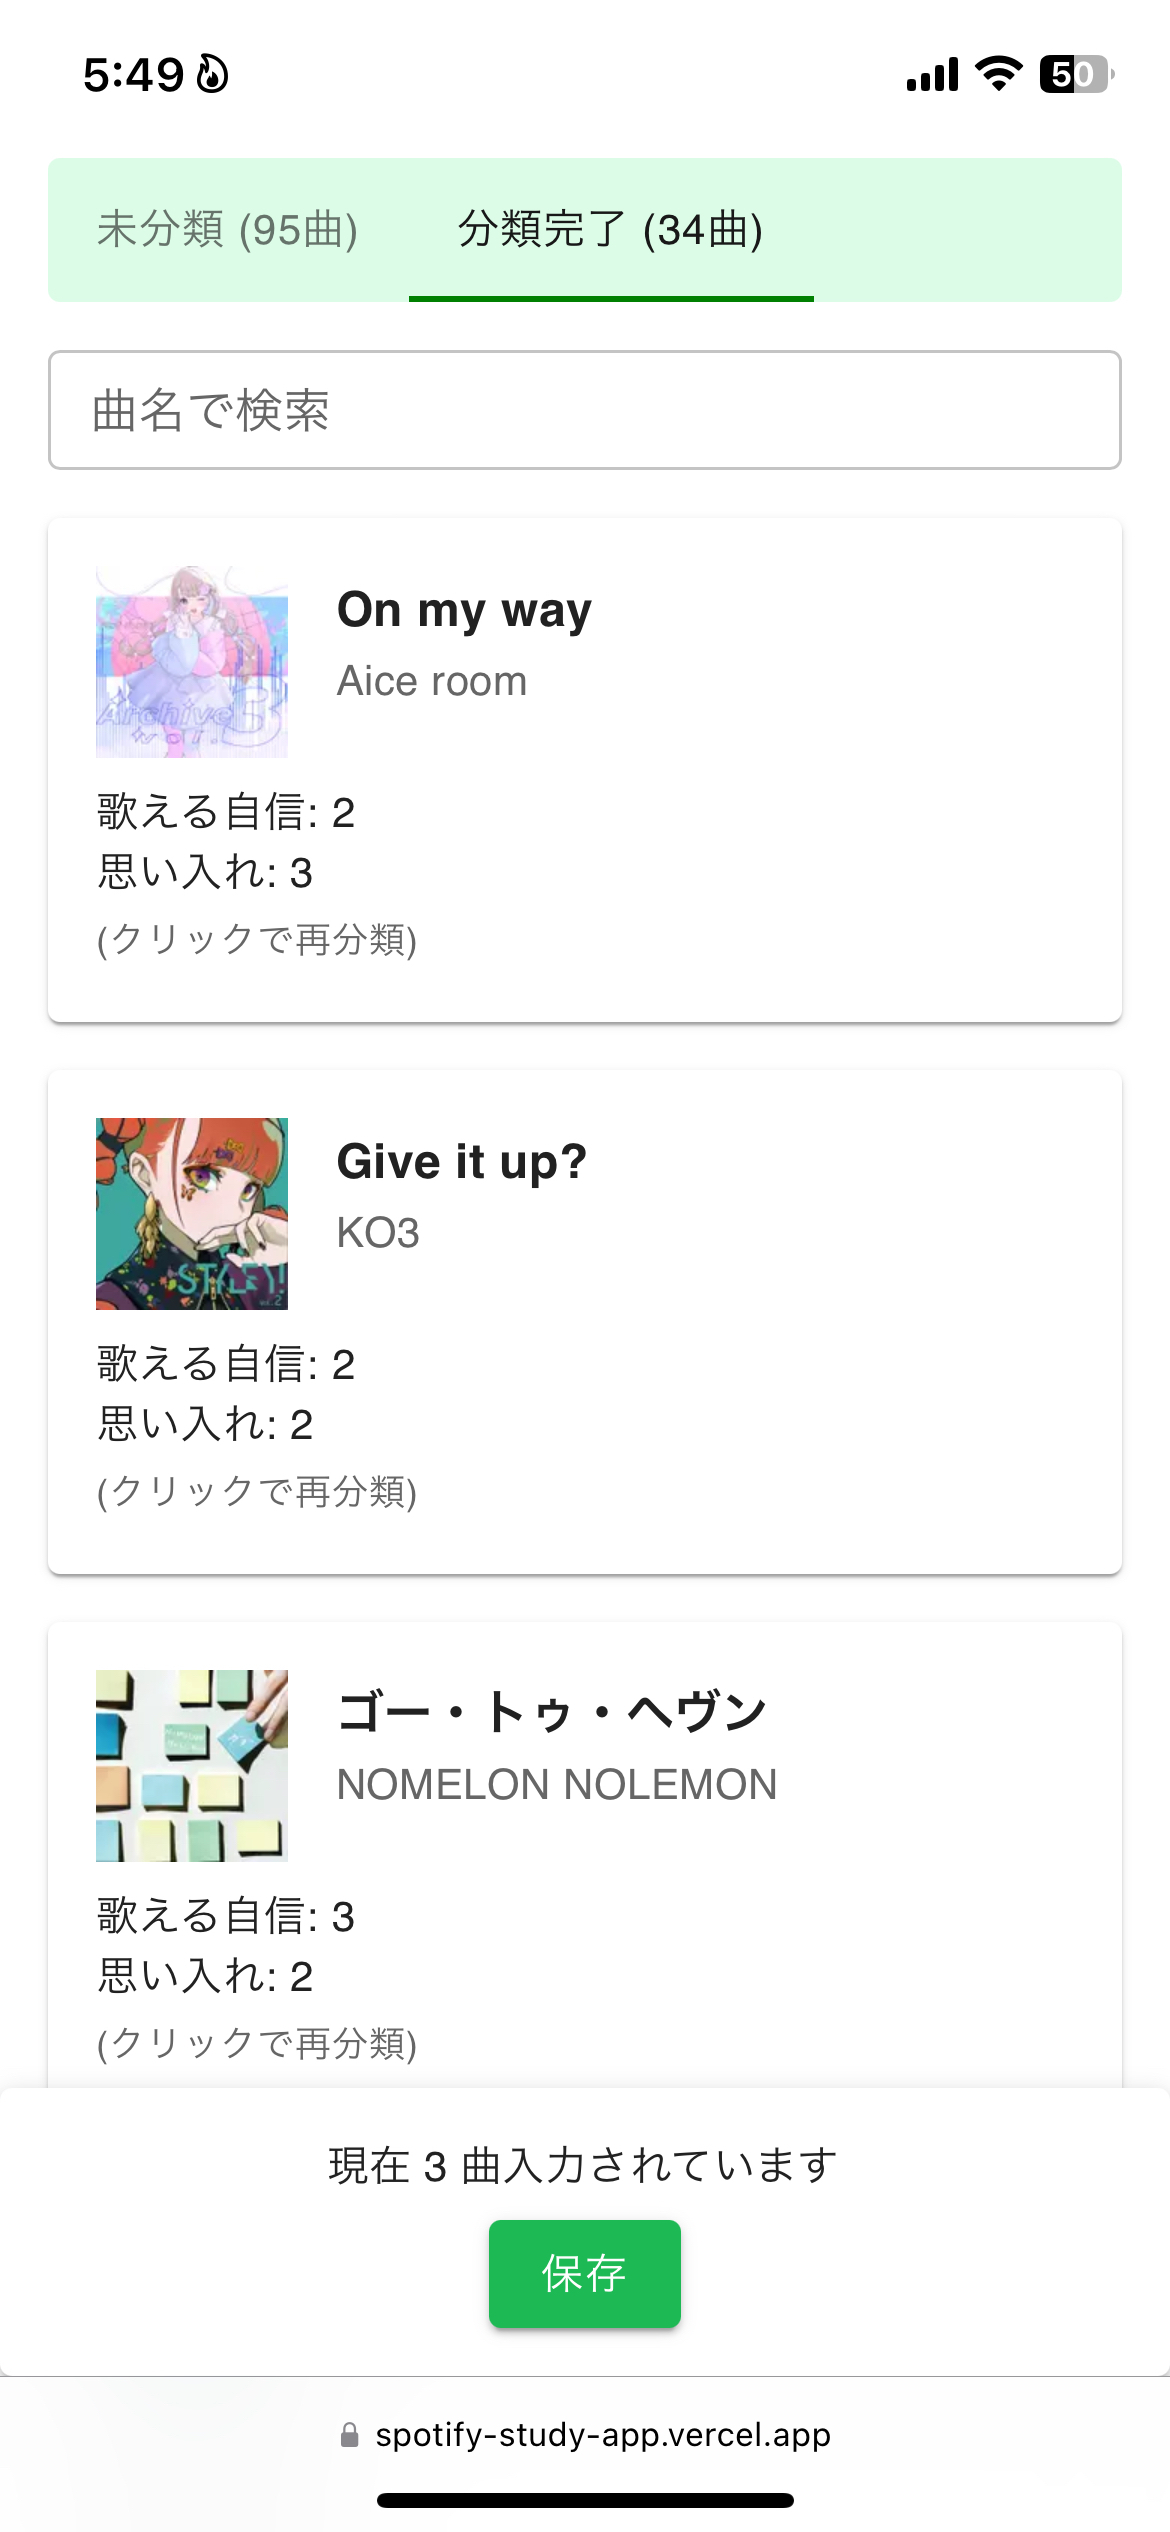
\includegraphics[width=0.9\linewidth]{image/ss_分類済み.png}
       \caption{分類済み楽曲一覧画面}
       \label{fig:classified_songs}
   \end{minipage}
\end{figure}


\subsection{本実験}

各被験者ペアを，本学の実験環境に案内し，互いに横並びになる形で座椅子に着席させる（図\ref{pic:実験環境}参照）．被験者に対して実験手順と注意点について説明し，音楽共有セッションを開始するよう指示をする．音楽共有セッションについては，以下の説明を行う．

\vskip.5\baselineskip

\textbf{推薦なし群:}
このセッションでは，あなたの音楽の好みについて相手と共有していただきます．
好きな曲をリストから選んで，選んだ曲を一緒に聴いたあと，その曲についてお話しください．曲にまつわる思い出や感想など，自由に会話を楽しんでください．

\vskip.5\baselineskip

\textbf{推薦あり群:}
このセッションでは，音楽を通じたコミュニケーションを体験していただきます．
システムが，あなたの音楽の興味や好みに基づいた曲の候補を提示します．
提示された候補の中から，共有したい曲を選んでください．
選んだ曲を一緒に聴いたあと，その曲についてお話しください．曲にまつわる思い出や感想など，自由に会話を楽しんでください．

\vskip.5\baselineskip

音楽共有セッションは全8フェーズで構成される．各フェーズは2ターン制を採用しており，以下の流れで進行する：

\begin{itemize}
    \item 第1ターン：被験者Aが開示者となり，被験者Bが被開示者となる
    \item 第2ターン：被験者Bが開示者となり，被験者Aが被開示者となる
\end{itemize}

つまり，1フェーズは「被験者A→被験者B」「被験者B→被験者A」という順序で2回の自己開示が行われる．

各ターンは，以下の3つのステップにより構成される．

\begin{enumerate}
    \item 楽曲選択フェーズ（30秒）
    \begin{itemize}
        \item 推薦なし群：事前に作成した個人のプレイリストから任意の1曲を選択する（図\ref{fig:free_selection}）
        \item 推薦あり群：システムが推薦する4曲の中から1曲を選択する（図\ref{fig:recommendation}）
    \end{itemize}
    
    \item 楽曲再生フェーズ（30秒）
    \begin{itemize}
        \item 選択楽曲を再生する．開示者が好きな場所から再生することができる
    \end{itemize}
    
    \item 対話フェーズ（60-90秒）
    \begin{itemize}
        \item 選曲理由や楽曲にまつわる思い出などを自由に共有し対話する
    \end{itemize}
    
\end{enumerate}

1フェーズが終わるごとに，GoogleForms\cite{googleforms}を利用して開示者と被開示者の双方が評価を行う．

\vskip.5\baselineskip

\begin{figure}[H]
    \centering
    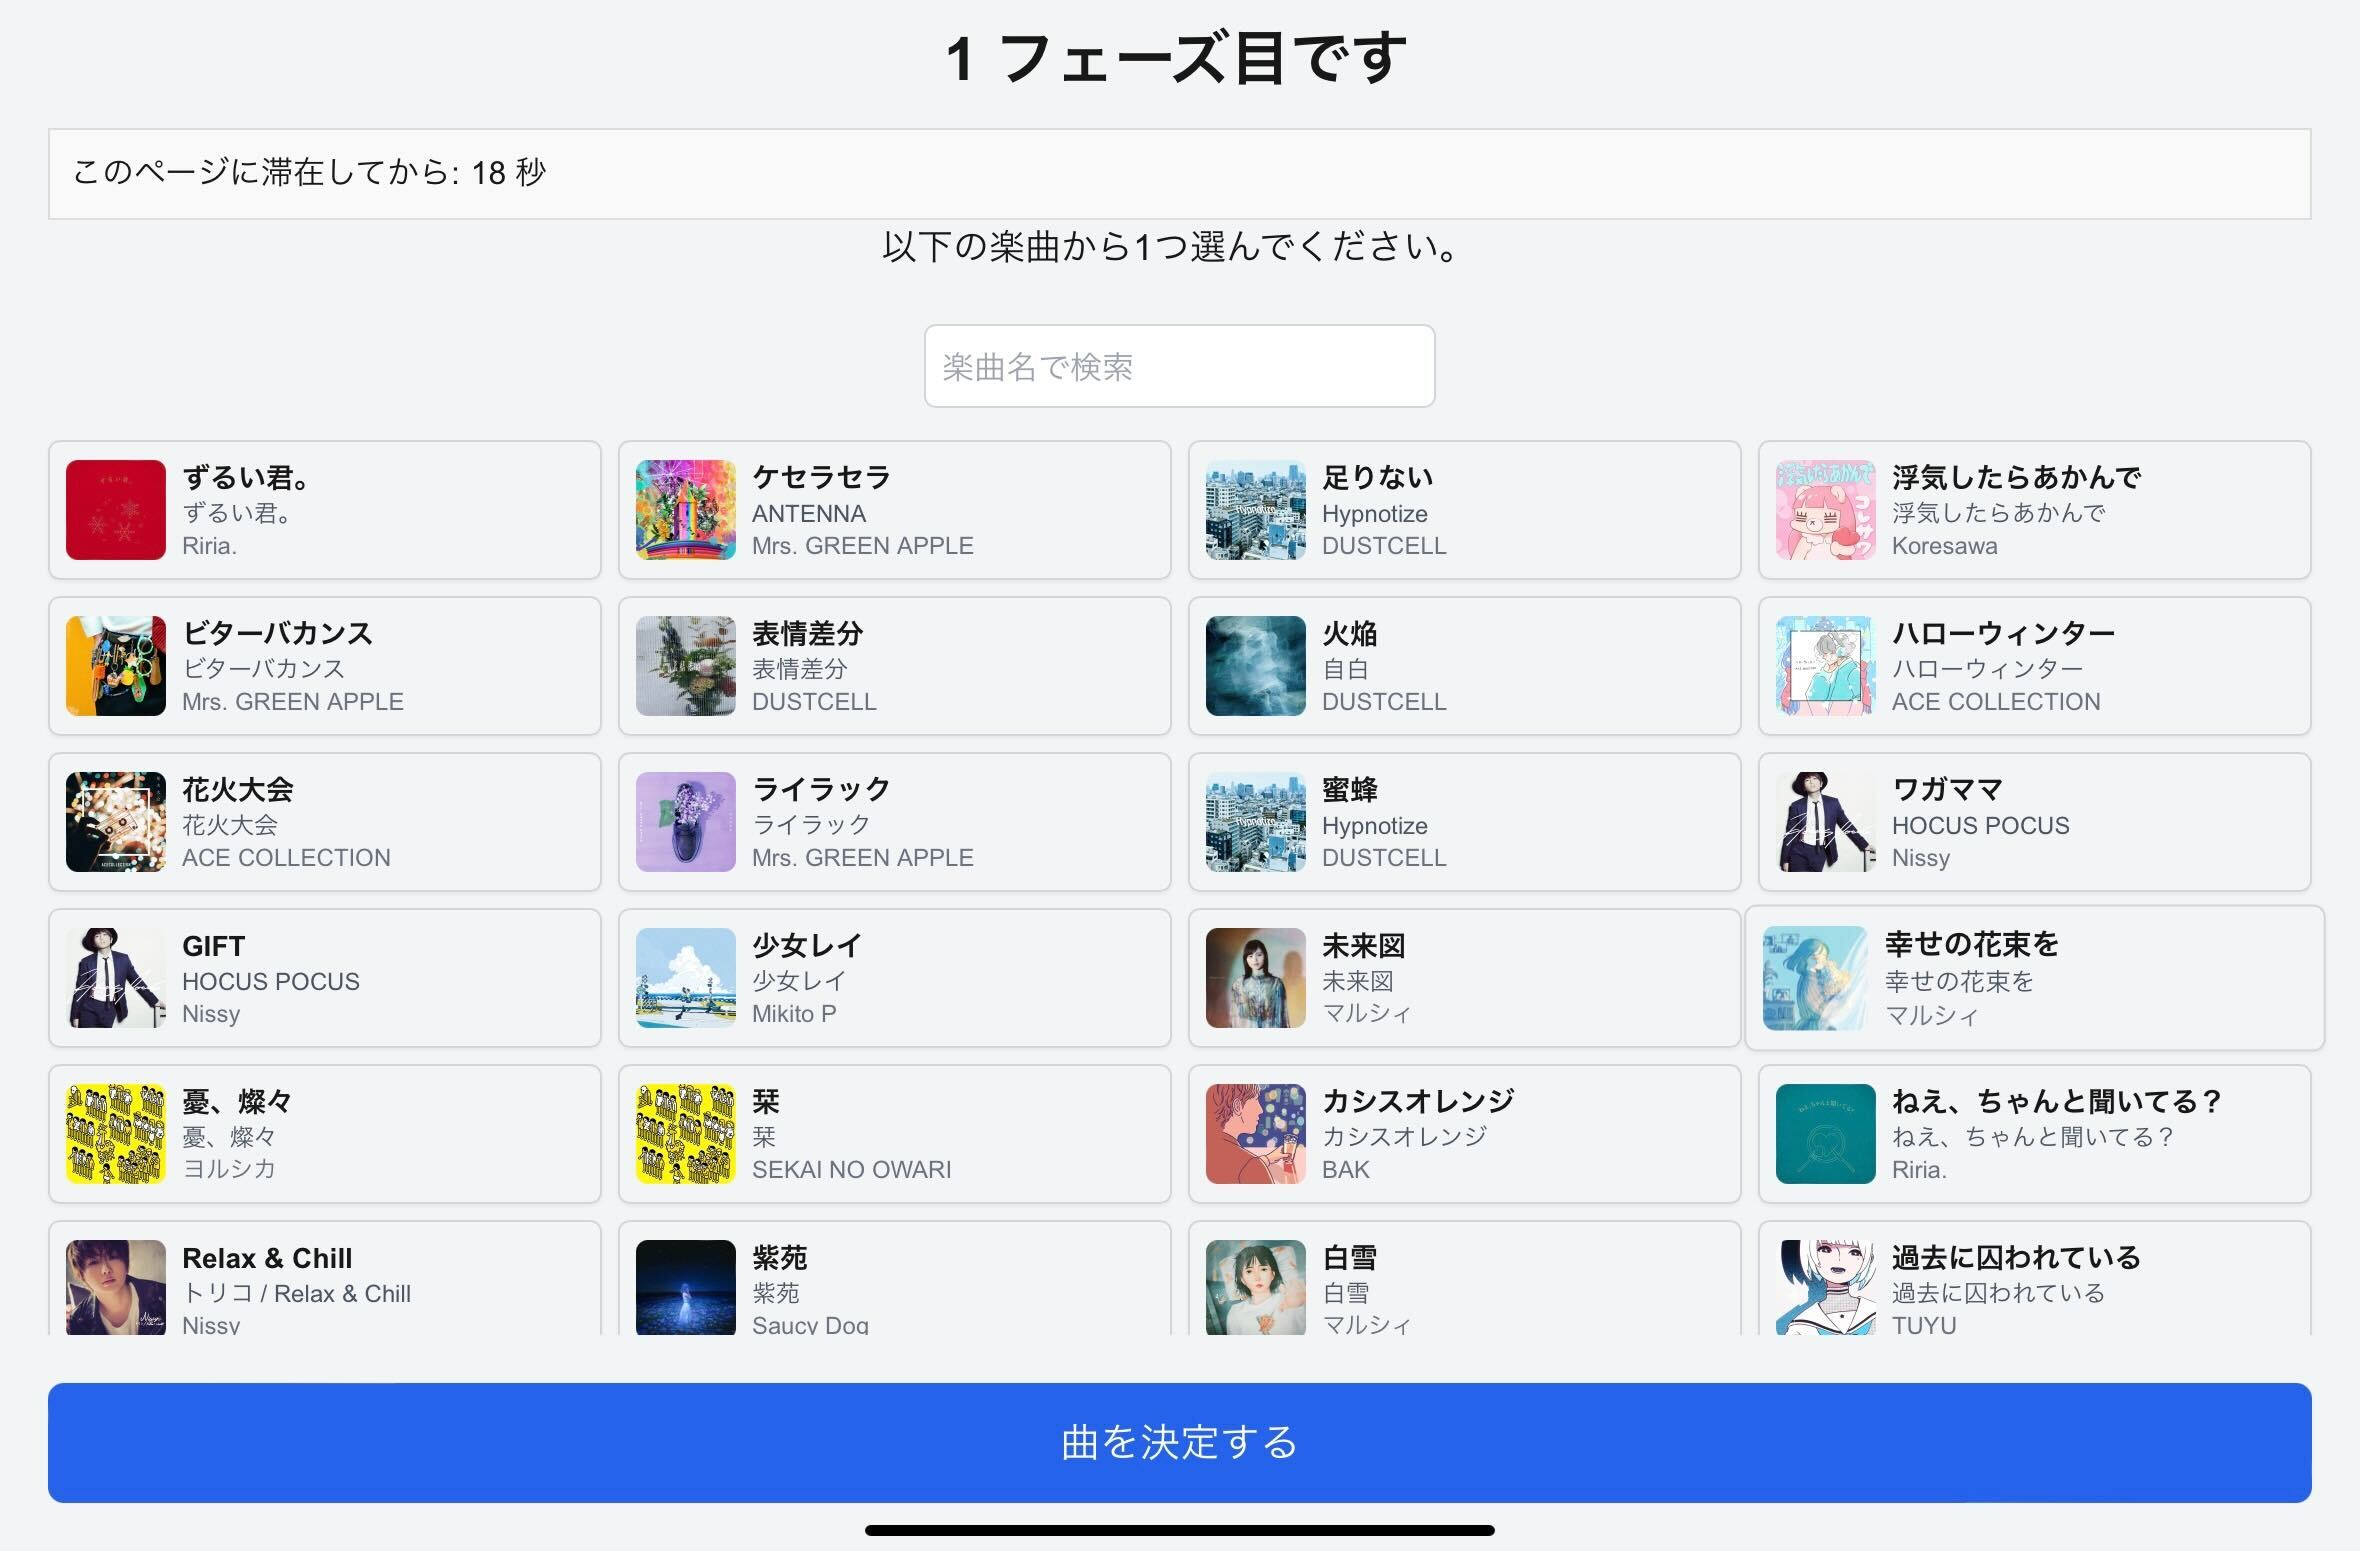
\includegraphics[width=0.9\linewidth]{image/ss_推薦なし_選曲.png}
    \caption{自由選択画面（推薦なし群）}
    \label{fig:free_selection}
\end{figure}

\begin{figure}[H]
    \centering
    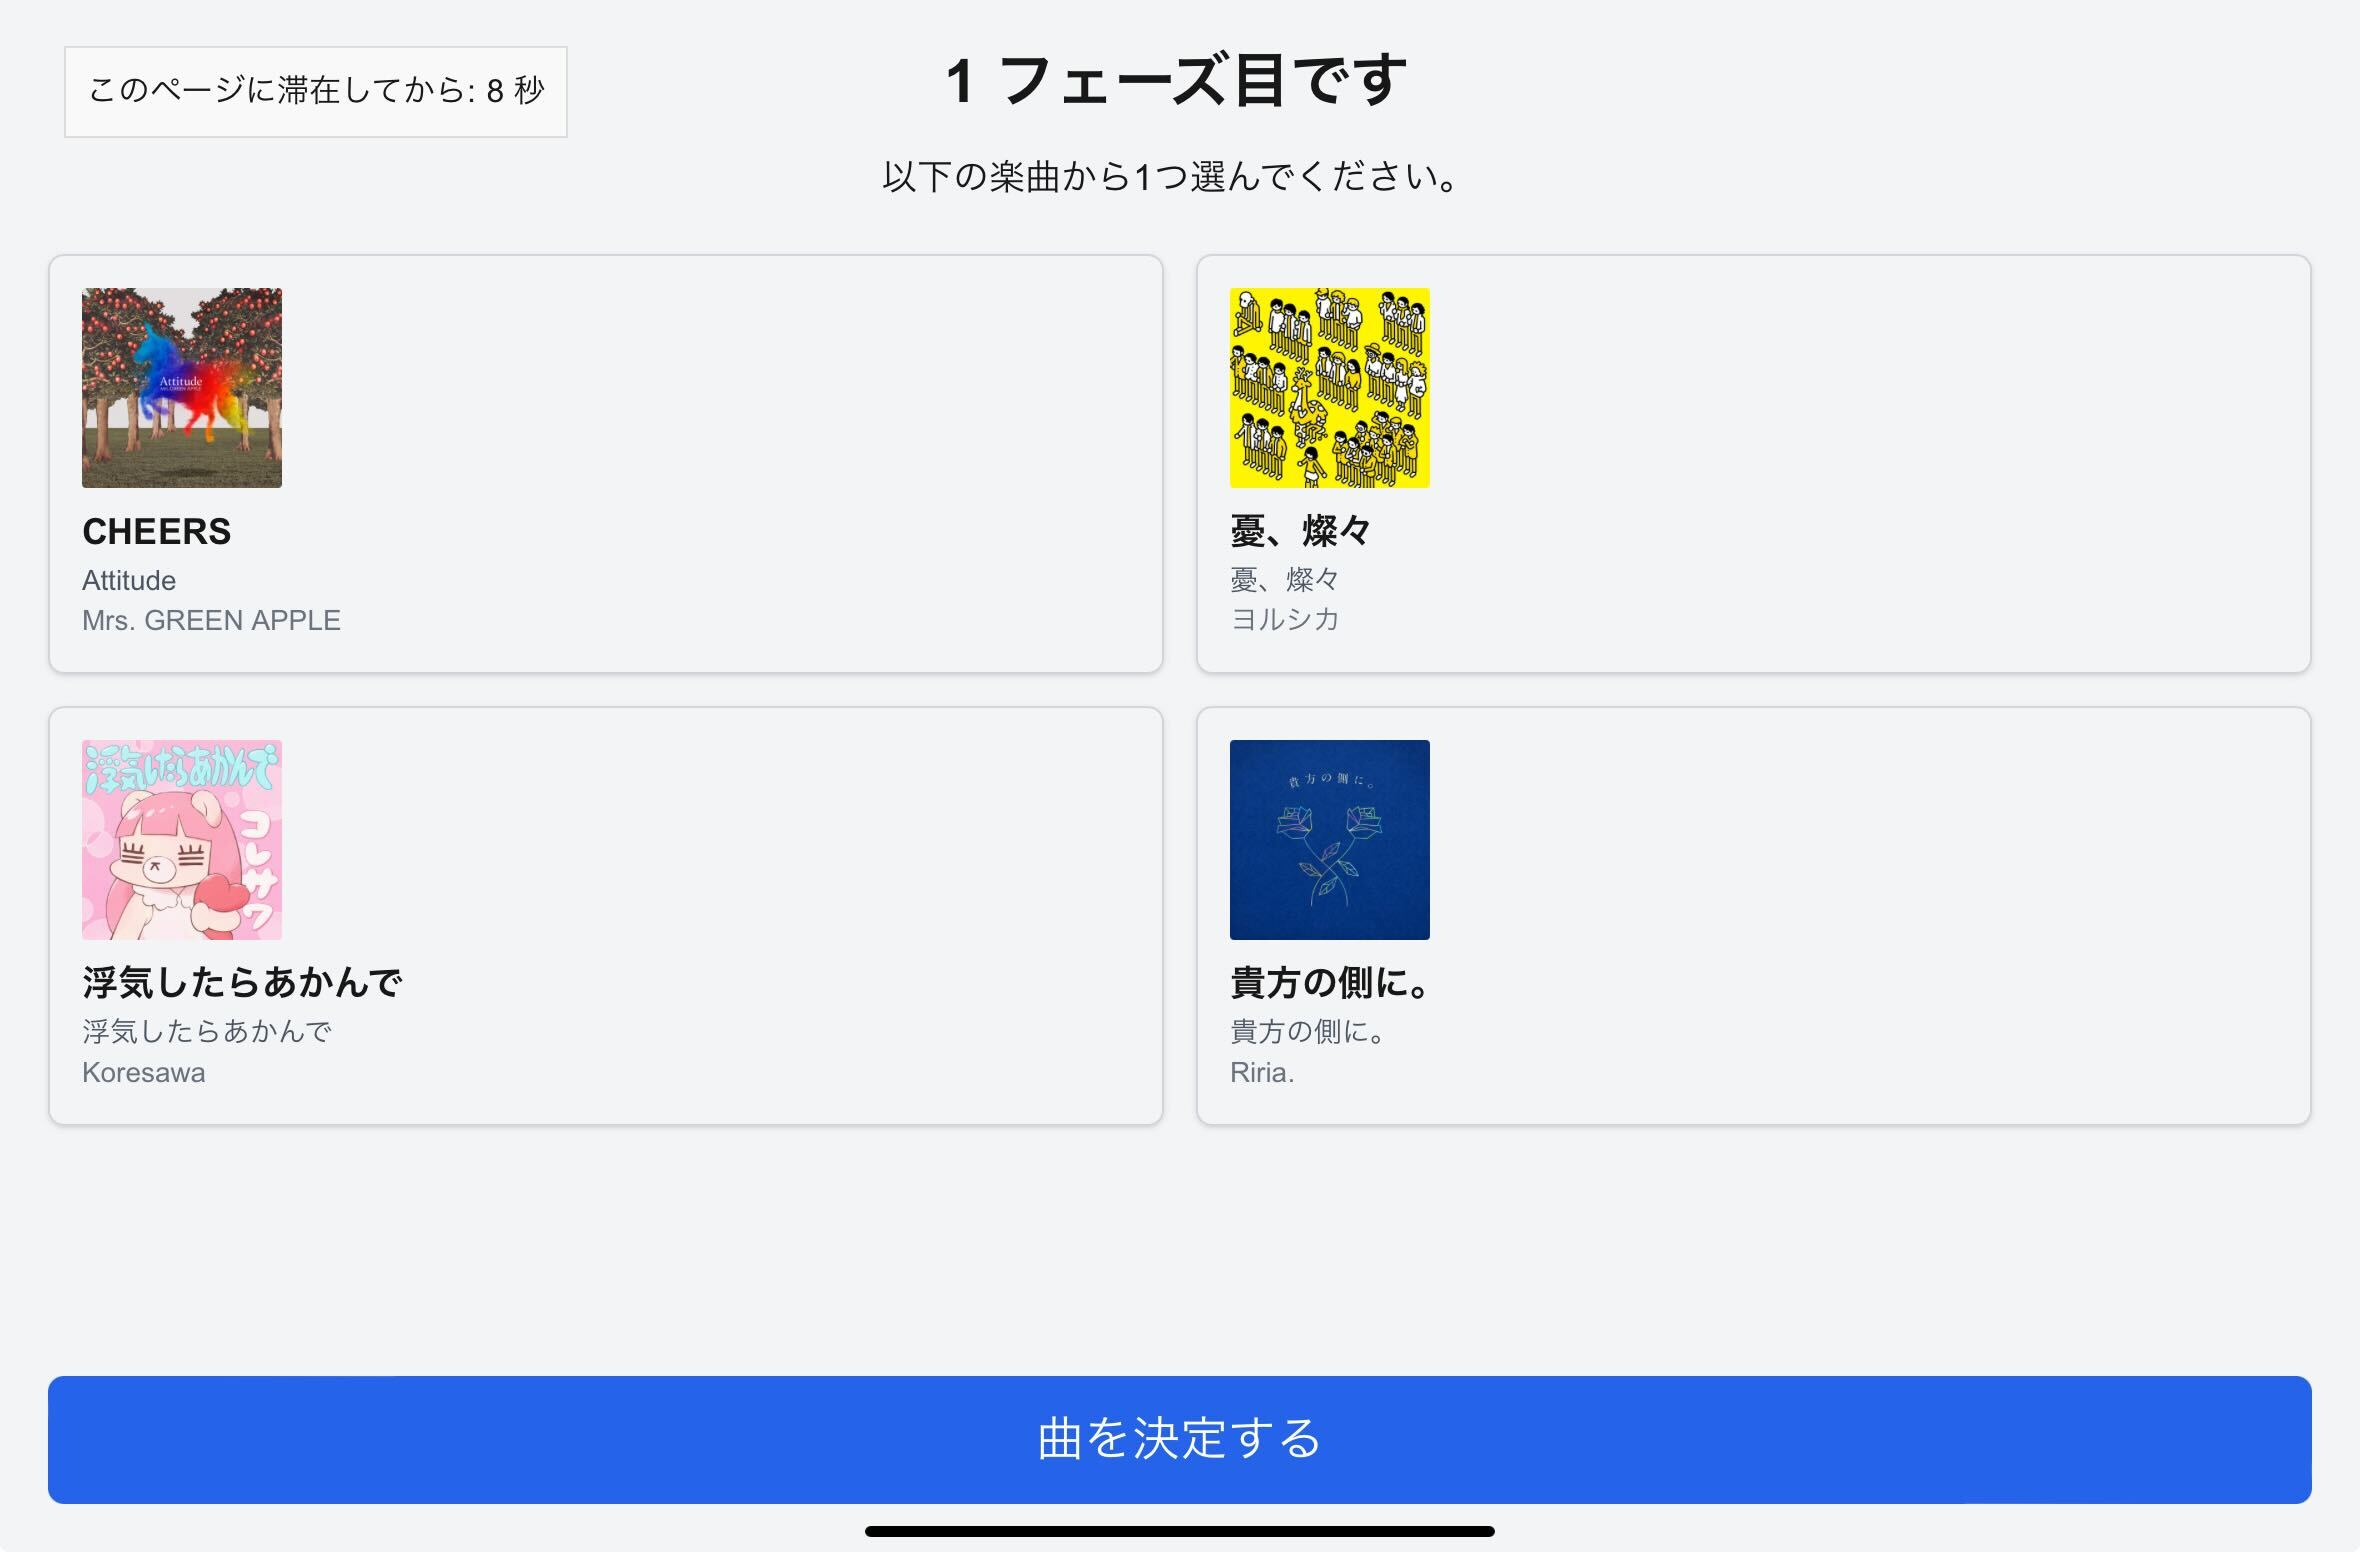
\includegraphics[width=0.9\linewidth]{image/ss_推薦あり_選曲.png}
    \caption{楽曲推薦画面（推薦あり群）}
    \label{fig:recommendation}
\end{figure}


% \subsection*{注意点}
% あとでくわしくかく
